% Digital Logic Lab 8 4-Digit Display
% Created: 2020-03-25, Ashlie Lackey and Megan Gordon

%==========================================================
%=========== Document Setup  ==============================

% Formatting defined by class file
\documentclass[11pt]{article}

% ---- Document formatting ----
\usepackage[margin=1in]{geometry}	% Narrower margins
\usepackage{booktabs}				% Nice formatting of tables
\usepackage{graphicx}				% Ability to include graphics

%\setlength\parindent{0pt}	% Do not indent first line of paragraphs 
\usepackage[parfill]{parskip}		% Line space b/w paragraphs
%	parfill option prevents last line of pgrph from being fully justified

% Parskip package adds too much space around titles, fix with this
\RequirePackage{titlesec}
\titlespacing\section{0pt}{8pt plus 4pt minus 2pt}{3pt plus 2pt minus 2pt}
\titlespacing\subsection{0pt}{4pt plus 4pt minus 2pt}{-2pt plus 2pt minus 2pt}
\titlespacing\subsubsection{0pt}{2pt plus 4pt minus 2pt}{-6pt plus 2pt minus 2pt}

% ---- Hyperlinks ----
\usepackage[colorlinks=true,urlcolor=blue]{hyperref}	% For URL's. Automatically links internal references.

% ---- Code listings ----
\usepackage{listings} 					% Nice code layout and inclusion
\usepackage[usenames,dvipsnames]{xcolor}	% Colors (needs to be defined before using colors)

% Define custom colors for listings
\definecolor{listinggray}{gray}{0.98}		% Listings background color
\definecolor{rulegray}{gray}{0.7}			% Listings rule/frame color

% Style for Verilog
\lstdefinestyle{Verilog}{
	language=Verilog,					% Verilog
	backgroundcolor=\color{listinggray},	% light gray background
	rulecolor=\color{blue}, 			% blue frame lines
	frame=tb,							% lines above & below
	linewidth=\columnwidth, 			% set line width
	basicstyle=\small\ttfamily,	% basic font style that is used for the code	
	breaklines=true, 					% allow breaking across columns/pages
	tabsize=3,							% set tab size
	commentstyle=\color{gray},	% comments in italic 
	stringstyle=\upshape,				% strings are printed in normal font
	showspaces=false,					% don't underscore spaces
}

% How to use: \Verilog[listing_options]{file}
\newcommand{\Verilog}[2][]{%
	\lstinputlisting[style=Verilog,#1]{#2}
}




%======================================================
%=========== Body  ====================================
\begin{document}

\title{ELC 2137 Lab 8: 4-Digit Display}
\author{Ashlie Lackey and Megan Gordon}

\maketitle


\section*{Summary}

Type the summary of your experiment and results here.  


\section*{Q\&A}

Answer questions posed in the lab assignment here.


\section*{Results}

In this section, put your simulation waveforms, results tables, pictures of hardware, and any other required items.

\begin{figure}[ht]\centering
	\begin{tabular}{l|rrrr}
		Time (ns): & 0 & 10 & 20 & 30 \\
		\midrule
		in0 & 00 & 01 & 10 & 10 \\
		in1 & 01 & 10 & 01 & 01 \\
		sel & 0 & 1 & 0 & 1 \\
		\midrule
		out & 00 & 10 & 10 & 01 \\
		\bottomrule
	\end{tabular}\medskip

	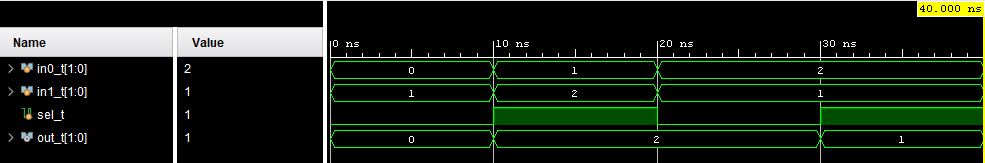
\includegraphics[width=1.1\textwidth]{mux2sim.png}
	\caption{Mux2 ERT and Testbench Results}
	\label{fig:sim_with_table}
\end{figure}
\clearpage

\begin{figure}[ht]\centering
	\begin{tabular}{l|rrrr}
		Time (ns): & 0 & 10 & 20 & 30 \\
		\midrule
		in0 & 0000 & 0000 & 0000 & 0000 \\
		in1 & 0001 & 0001 & 0001 & 0001 \\
		in2 & 0010 & 0010 & 0010 & 0010 \\
		in3 & 0011 & 0011 & 0011 & 0011 \\
		sel & 00 & 01 & 10 & 11 \\
		\midrule
		out & 0000 & 0001 & 0010 & 0011 \\
		\bottomrule
	\end{tabular}\medskip
	
	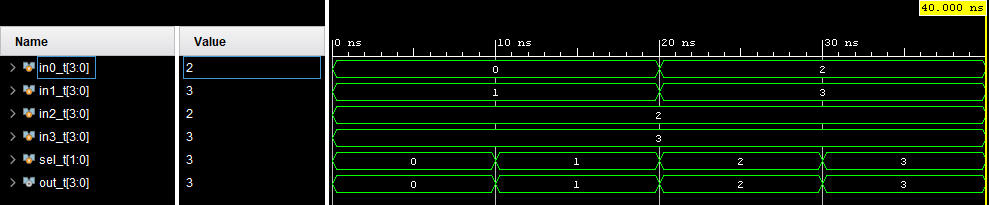
\includegraphics[width=1.1\textwidth]{mux4sim.png}
	\caption{Mux4 ERT and Testbench Results}
	\label{fig:sim_with_table}
\end{figure}

\begin{figure}[ht]\centering
	\begin{tabular}{l|rrrr}
		Time (ns): & 0 & 10 & 20 & 30 \\
		\midrule
		in0 & 00 & 01 & 10 & 11 \\
		\midrule
		out & 1110 & 1101 & 1011 & 0111 \\
		\bottomrule
	\end{tabular}\medskip

	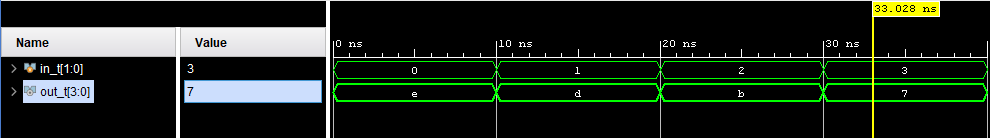
\includegraphics[width=1.1\textwidth]{an_decodesim.png}
	\caption{an-decoder ERT and Testbench Results}
	\label{fig:sim_with_table}
\end{figure}

\section*{Code}

Code for mux2, mux4, andecode, sseg4, sseg4manual is included below.

\begin{lstlisting}[style=Verilog,caption=Mux2 Module Code,label=code:ex ]
`timescale 1ns / 1ps
// Ashlie Lackey and Megan Gordon, ELC 2137, 2020 -03 -05
module mux2 #(parameter N=2)(input [N-1:0]in0, [N-1:0]in1, 
	input sel,
	output [N-1:0]out);
	
	assign out = sel?in1:in0;
endmodule
\end{lstlisting}

\begin{lstlisting}[style=Verilog,caption=Mux4 Module Code,label=code:ex ]
`timescale 1ns / 1ps
// Ashlie Lackey and Megan Gordon, ELC 2137, 2020 -03 -05

module mux4 #(parameter N=4)(input [N-1:0] in3, 
							input [N-1:0] in2, 
							input [N-1:0] in1, 
							input [N-1:0] in0,
							input [1:0] sel,
							output reg [N-1:0] out);
	always @(*)
	begin
		case(sel)
		0: out = in0;
		1: out = in1;
		2: out = in2;
		default: out = in3;
		endcase;
	end
endmodule
\end{lstlisting}

\begin{lstlisting}[style=Verilog,caption=andecoder Module Code,label=code:ex ]
`timescale 1ns / 1ps
// Ashlie Lackey and Megan Gordon, ELC 2137, 2020 -03 -05

module an_decode(input [1:0] in,
	output reg [3:0] out);
	
	always @*
		begin
			case(in)
			0: out = 4'b1110;
			1: out = 4'b1101;
			2: out = 4'b1011;
			default: out = 4'b0111;
			endcase
		end
endmodule
\end{lstlisting}

\begin{lstlisting}[style=Verilog,caption=sseg4 Module Code,label=code:ex ]
`timescale 1ns / 1ps
// Ashlie Lackey and Megan Gordon, ELC 2137, 2020 -03 -05

module sseg4(input [15:0] data,
			input hex_dec,sign,
			input [1:0] digit_sel,
			output reg [7:0] seg,
			output reg dp,
			output reg [3:0] an);

	wire [15:0] bcd11out;
	bcd11 sseg4_bcd11(.B(data[10:0]), .Boutfinal(bcd11out));
	
	wire [15:0] mux2_1_out;
	mux2 #(.N(16))sseg4_mux2_1(.in0(bcd11out), .in1(data[15:0]), .sel(hex_dec), .out(mux2_1_out));
	
	wire [3:0] mux4_out;
	mux4 sseg4_mux4(.in0(mux2_1_out[3:0]), .in1(mux2_1_out[7:4]),.in2(mux2_1_out[11:8]), .in3(mux2_1_out[15:12]), .sel(digit_sel), .out(mux4_out));
	
	wire [6:0]sseg_decoder_out;
	sseg_decoder sseg4_decode(.num(mux4_out), .sseg(sseg_decoder_out));
	
	wire [3:0] decoder_out;
	an_decode an_decode_sseg4(.in(digit_sel), .out(decoder_out));
	
	wire mux22_in;
	assign mux22_in = ~decoder_out[3] & sign;
	mux2 #(.N(7)) sseg4_mux2_2(.in0(sseg_decoder_out), .in1(7'b0111111), .sel(mux22_in), .out(seg));
	
	assign dp = 1;
	assign an = decoder_out;

endmodule
\end{lstlisting}

\begin{lstlisting}[style=Verilog,caption=sseg4 manual Module Code,label=code:ex ]
`timescale 1ns / 1ps
// Ashlie Lackey and Megan Gordon, ELC 2137, 2020 -03 -05

module sseg4_manual(input [15:0]sw,
					output [6:0] seg,
					output dp,
					output [3:0] an);
	
	sseg4 boardconnect(.data({4'b0000, sw[11:0]}), .hex_dec(sw[15]), .sign(sw[14]), .digit_sel(sw[13:12]), .seg(seg), .dp(dp), .an(an));              
endmodule
\end{lstlisting}

\end{document}
